\section{Gnuplot \textcolor{red}{(unfinished)}}

\newcounter{gnuplothomework} \newcommand{\gphome}{\begin{large}Homework \arabic{gnuplothomework}\end{large}}
\newcounter{gnuplotexample}  \newcommand{\gpexample}{Example \arabic{gnuplotexample}}

% \vspace*{-1cm}
% \begin{flushright}
% \texttt{set term classnotes}
% \end{flushright}

Gnuplot is a tradicional, very useful and powerful tool for scientific plot. It can be used either for quick plots to visualize data, or to obtain fine figures for reports and publications. Gnuplot's current version at the time I'm writing these notes is \texttt{5.0}, and it can be found on the webpage \url{www.gnuplot.info}. There one also finds an extensive User Manual. In this chapter we elaborate on the main aspects of \texttt{gnuplot} to introduce the language and capabilities of this fantastic tool for the students.

\subsection{Installing gnuplot}

\subsection*{Debian/Ubuntu Linux}

Most Linux distributions have \texttt{gnuplot} in their repositories. If you use Ubuntu, you can install from the terminal with the commands:

\begin{example}{Installing gnuplot in Ubuntu Linux}
\begin{minted}[]{bash}
 sudo apt-get update
 sudo apt-get install gnuplot # this installs gnuplot version 4.6.6
 # or...
 sudo apt-get install gnuplot5 # this installs gnuplot version 5.0
 sudo apt-get install gnuplot-mode # To install gnuplot emacs mode
\end{minted}
\end{example}

If you use the \texttt{Emacs} text editor, the \texttt{gnuplot-mode} package above provides a full IDE for \texttt{gnuplot} within \texttt{Emacs}.

\subsection*{MS Windows and Apple OS X}

I highly recommend you to use \texttt{Linux}. However, if you are stubborn enough I allow you to waste time with another OS. If you have an Apple computer (at least that's UNIX-based) you can install \texttt{gnuplot} via \texttt{homebrew}\footnote{Homebrew: \url{brew.sh}.} or \texttt{MacPorts}\footnote{MacPorts: \url{www.macports.org}.}. If you use Windows (really?)... good luck!


\subsection{The command line interface}

\texttt{Gnuplot} runs on the command line, there's no GUI. If you really like graphical interfaces, please check \texttt{QtiPlot}\footnote{QtiPlot: \url{www.qtiplot.com}.}. To start \texttt{gnuplot} (in \texttt{Linux}) open the terminal, type \texttt{gnuplot} and press Enter... you will see this interface:

\begin{example}{Gnuplot's initial screen}
\begin{minted}{bash}
        G N U P L O T                                                                                                             
        Version 5.0 patchlevel 1    last modified 2015-06-07                                                                      
                                                                                                                                  
        Copyright (C) 1986-1993, 1998, 2004, 2007-2015                                                                                
        Thomas Williams, Colin Kelley and many others

        gnuplot home:     http://www.gnuplot.info
        faq, bugs, etc:   type "help FAQ"
        immediate help:   type "help"  (plot window: hit 'h')

Terminal type set to 'qt'
gnuplot> 
\end{minted}
\end{example}

From the start it tells you that if you need help, just type \texttt{help}. In \texttt{gnuplot} this is extremely useful, as it comes with an extensive and well written documentation. Therefore, let's start with the most important command: \mintinline[escapeinside=||]{gnuplot}{|gnuplot>| help plot}. Read it! Check and test the examples by yourself.

In the examples you will see that you can call sine and cosine functions natively. Actually, \texttt{gnuplot} supports all functions from the Unix math library. When in doubt try common names for the functions. For instance, let's try to plot a Gaussian:

\begin{example}{Plotting Gaussians with gnuplot}
\begin{minted}[escapeinside=||]{gnuplot}
 |gnuplot>| w = 2.0; # set variable w to store the Gaussian width
 |gnuplot>| set xrange [-10:10]; # set the range of horizontal axes
 |gnuplot>| f(x)=exp(-0.5*(x/w)**2); # define a Gaussian function
 |gnuplot>| plot f(x); # plot f(x)
 |gnuplot>| plot f(x), f(x-1); # plot two functions
\end{minted}
\end{example}

Try to run this example line-by-line in \texttt{gnuplot}. If all goes well you should get Fig.~\ref{fig:gnuplotgaussian}. Excellent! Now you understand how the \texttt{gnuplot} interface works and you made your first plot. Play around and try to plot other functions, change the axes range and read again the plot help to see what you can do. By default you are probably using the `qt' terminal, which allows you to save, copy and print your figure from the plot window.

\begin{figure}[ht!]
 \centering
 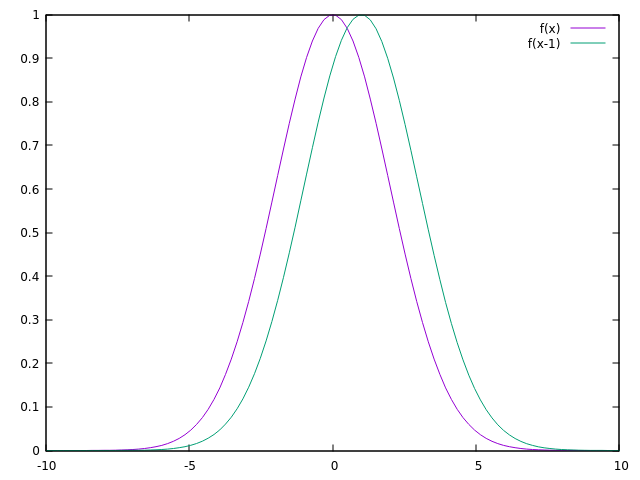
\includegraphics[width=0.5\textwidth]{gnuplot-gaussian.png}
 \caption{Plot of Gaussian functions in \texttt{gnuplot}.}
 \label{fig:gnuplotgaussian}
\end{figure}

\subsection{Using a script file}

While the command line interface is very useful for quick plots, for final figures you will probably need to customize colors, styles, sizes, labels... this can be easily accomplished using a script file, which is simply a text file containing all the commands you want to run. Using your favorite text editor create a file \texttt{gaussian.gp} with the content:

\begin{example}{gnuplot script file `gaussian.gp'}
\begin{minted}[]{gnuplot}
  reset; # cleans the variables and functions
  w = 2.0; # set variable w to store the Gaussian width
  f(x)=exp(-0.5*(x/w)**2); # define a Gaussian function
  set xrange [-10:10]; # set the range of horizontal axes
  set yrange [-0.1:1.1]; # set the range of vertical axes
  set title 'Gaussians'
  set xlabel 'here goes x'
  set ylabel 'here goes f(x)'
  plot f(x) lw 4, f(x-1) lw 2; # plot two functions
\end{minted}
\end{example}

From the \texttt{gnuplot} interface call: \mintinline[escapeinside=||]{gnuplot}{|gnuplot>| load 'gaussian.gp'}. It will open a plot window similar to the previous one, check the differences to understand the new commands on the example.

\subsection{The terminals}

\subsubsection{Example script: epslatex}

\subsection{Using gnuplot with Julia}

\subsection{Most useful commands and examples}

% \section{Another choice: Asymptote}


